\documentclass[14pt,a4paper]{extarticle}
\usepackage[T2A]{fontenc}
\usepackage[utf8]{inputenc}
\usepackage[english,russian]{babel}
\usepackage{lmodern}
\usepackage{geometry}
\usepackage{array}
\usepackage{tabularx}
\usepackage{longtable}
\usepackage{ltablex}
\usepackage{booktabs}
\usepackage{hyperref}
\usepackage{indentfirst}
\usepackage{microtype}
\usepackage{graphicx}
\usepackage{setspace}
\usepackage{listings}
\usepackage{graphicx}
\usepackage{caption}
\usepackage{float}
\usepackage{tocloft}
\usepackage{titlesec}
\usepackage{newtxtext,newtxmath}

\titleformat{\section}        % форматируем \section
  {\normalfont\bfseries}      % стиль: обычный + жирный
  {\thesection.}              % номер секции с точкой
  {2mm}                       % расстояние между номером и текстом
  {}                           % перед заголовком можно добавить что-то
\titlespacing*{\section}{1.5cm}{*3}{*1}  % {отступ слева}{отступ сверху}{отступ снизу}

\captionsetup{justification=centering}
\renewcommand{\ttdefault}{cmtt}
\keepXColumns
\setlength{\parindent}{3em}
\newgeometry{left=2.5cm,right=2.5cm,top=3cm,bottom=2.5cm}

\renewcommand{\contentsname}{\hspace*{4em}{\smallСодержание}}
\setlength{\cftbeforesecskip}{0.5em}
\renewcommand{\cftsecleader}{\cftdotfill{\cftdotsep}}
\renewcommand{\cftsecaftersnum}{.\hspace{2mm}}

\title{Отчёт по дисциплине "Системная инженерия"}
\author{Выполнил студент группы М-РИТ-25-1, Станиславчук Сергей}

\begin{document}

\setstretch{1.5}
\noindent
\begin{minipage}[t]{0.01\textwidth}
    \includegraphics{~/programmer/++Programmer/5_1/LSTU.jpg}
\end{minipage}%
\begin{minipage}[c]{1.1\linewidth}
    \centering
    {\small
    МИНИСТЕРСТВО НАУКИ И ВЫСШЕГО ОБРАЗОВАНИЯ РФ \\[1em]
    ФЕДЕРАЛЬНОЕ ГОСУДАРСТВЕННОЕ БЮДЖЕТНОЕ \\
    ОБРАЗОВАТЕЛЬНОЕ УЧРЕЖДЕНИЕ ВЫСШЕГО ОБРАЗОВАНИЯ \\
    «ЛИПЕЦКИЙ ГОСУДАРСТВЕННЫЙ ТЕХНИЧЕСКИЙ УНИВЕРСИТЕТ»
    }
\end{minipage}%

\vspace{3em}

\noindent
\hspace{1em}%
\begin{minipage}[t]{0.8\textwidth}
\textbf{Институт} \hspace{2em} компьютерных наук \\
\textbf{Кафедра} \hspace{2em} автоматизированных систем управления
\end{minipage}


\vspace{6em}

\begin{center}
\textbf{Домашнее задание №3} \\
по дисциплине \\ <<Системная инженерия>>
\end{center}

\vspace{6em}

\noindent
\begin{tabular*}{\textwidth}{@{\extracolsep{\fill}} l c r }
    Студент М-РИТ-25-1 & \makebox[4cm]{\hrulefill} & Станиславчук С.М. \\[2em]
Руководитель & \\
Профессор, канд. тех. наук & \makebox[4cm]{\hrulefill} & Качановский Ю.П. \\
\end{tabular*}

\vfill
\begin{center}
    Липецк, 2026
\end{center}

\thispagestyle{empty}

\newpage
\tableofcontents
\newpage

\section{Задание кафедры}
\begin{sloppypar}
    1. Привести вербальное (словесное) описание проектируемой системы
    (размещения), удовлетворения (соответствия), проверки, а также связи происхождения,
    2. Построить диаграмму (диаграммы) требований, использую связи включения
    уточнения, копирования и отслеживания (по возможности).
    3. Определить акторов и все варианты использования системы, в том числе обычные
    (основные) взаимодействия каждого актора с системой, а также альтернативные и
    исключительные взаимодействия
    4. Построить модель вариантов использования в виде диаграммы, применяя связи
    ассоциации, включения и расширения (чтобы отделить обычное поведение от
    альтернативного и исключительного), а также связи обобщения/конкретизации (по
    возможности)
    5. Подготовить описания по основным вариантам использования (не менее 4)
    6. Используя диаграммы требований и вариантов использования, сформировать системные
    функциональные требования к системе, а также определить нефункциональные
    требования (по возможности).
\end{sloppypar}

\section{Описание проектируемой системы}

Система корпоративного обмена сообщениями в реальном времени
Предназначена для организации защищённой текстовой и голосовой связи внутри корпоративной сети без использования внешних централизованных сервисов, с минимальной зависимостью от внешней инфраструктуры.

Объектом управления является коммуникационная инфраструктура организации, включающая серверы, клиентские устройства пользователей и сетевые каналы передачи данных. С помощью клиентского приложения пользователь получает доступ к текстовым чатам, голосовым каналам и передаче файлов. Управление системой осуществляется через интерфейс, позволяющий создавать каналы связи, отправлять сообщения, подключаться к голосовым сессиям и обмениваться данными.

Внутри системы осуществляется постоянное установление и поддержание соединений между клиентами и сервером. Сервер обрабатывает входящие сообщения, управляет сессиями пользователей и обеспечивает маршрутизацию данных. Передача текстовых сообщений происходит в режиме реального времени, а голосовая связь реализуется через потоковую передачу данных с учётом минимизации задержек.

Система также выполняет контроль доступа и защиту данных. Аутентификация пользователей, шифрование передаваемой информации и разграничение прав доступа обеспечивают безопасность взаимодействия. При передаче файлов система контролирует целостность данных и управляет их доставкой между участниками.

Таким образом, система обеспечивает автоматизированное управление процессом корпоративной коммуникации, поддерживая стабильный обмен данными, безопасность и высокую скорость взаимодействия внутри сети организации.

\section{Диаграмма требований}

Диаграмма требований представлена на рисунке 1.

\begin{figure}[H]
    \label{fig:1}
    \centering
    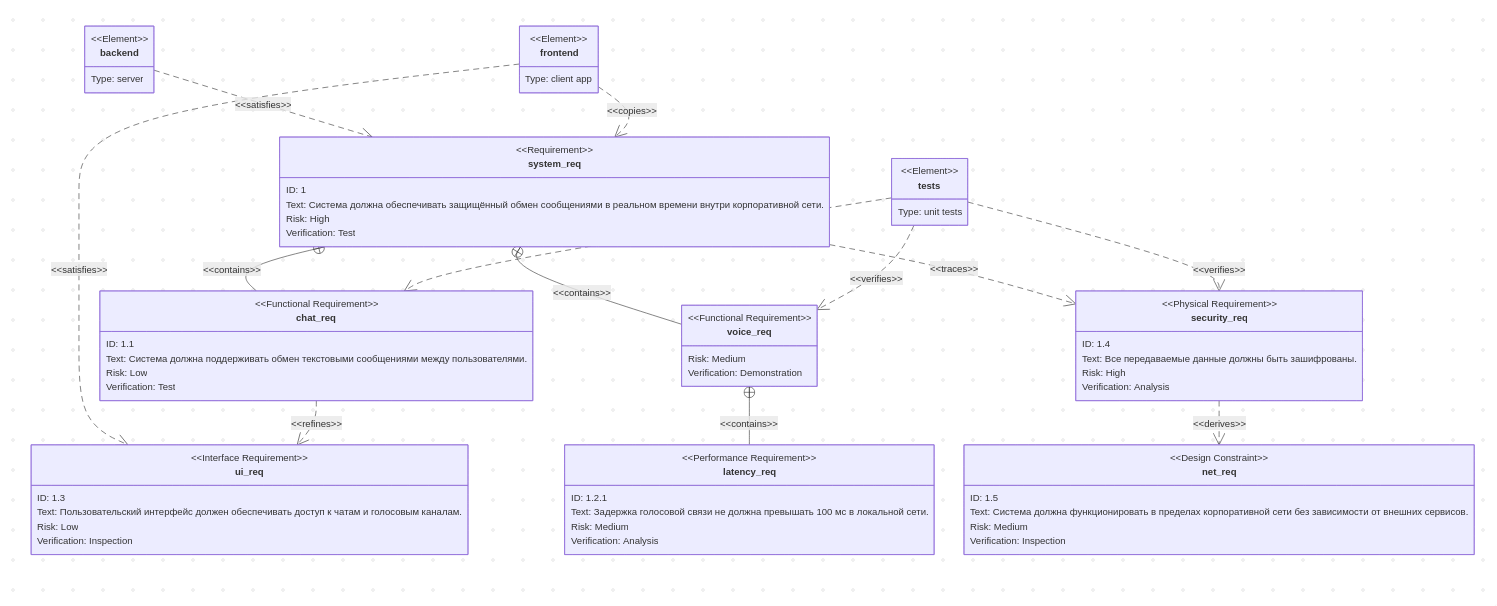
\includegraphics[width=0.78\textwidth]{req.png}
    \refstepcounter{figure}
    \caption*{Рисунок \thefigure\ — Диаграмма требований}
\end{figure}

\begin{verbatim}
requirementDiagram

requirement system_req {
    id: 1
    text: "Система должна обеспечивать защищённый обмен сообщениями в реальном времени внутри корпоративной сети."
    risk: high
    verifymethod: test
}

functionalRequirement chat_req {
    id: 1.1
    text: "Система должна поддерживать обмен текстовыми сообщениями между пользователями."
    risk: low
    verifymethod: test
}

functionalRequirement voice_req {
    id: 1.2
    text: "Система должна поддерживать голосовую связь в реальном времени."
    risk: medium
    verifymethod: demonstration
}

performanceRequirement latency_req {
    id: 1.2.1
    text: "Задержка голосовой связи не должна превышать 100 мс в локальной сети."
    risk: medium
    verifymethod: analysis
}

interfaceRequirement ui_req {
    id: 1.3
    text: "Пользовательский интерфейс должен обеспечивать доступ к чатам и голосовым каналам."
    risk: low
    verifymethod: inspection
}

physicalRequirement security_req {
    id: 1.4
    text: "Все передаваемые данные должны быть зашифрованы."
    risk: high
    verifymethod: analysis
}

designConstraint net_req {
    id: 1.5
    text: "Система должна функционировать в пределах корпоративной сети без зависимости от внешних сервисов."
    risk: medium
    verifymethod: inspection
}

element backend {
    type: server
}

element frontend {
    type: client app
}

element tests {
    type: unit tests
}

backend - satisfies -> system_req
frontend - satisfies -> ui_req

system_req - contains -> chat_req
system_req - contains -> voice_req
system_req - contains -> security_req

voice_req - contains -> latency_req

chat_req - refines -> ui_req

security_req - derives -> net_req

tests - verifies -> chat_req
tests - verifies -> voice_req
tests - verifies -> security_req

system_req - traces -> security_req

system_req <- copies - frontend

\end{verbatim}

\section{Акторы и варианты использования системы}

В проектируемой системе корпоративного обмена сообщениями выделяются три основных актора, взаимодействующих с системой на разных уровнях. Каждый актор характеризуется собственным набором функций и степенью вовлечённости в эксплуатацию системы.

Пользователь (сотрудник) является основным актором, непосредственно использующим функциональность системы для обмена сообщениями и организации коммуникации. Администратор системы отвечает за эксплуатационное сопровождение, управление инфраструктурой и пользователями. Специалист по информационной безопасности выполняет функции контроля защищённости системы, анализа инцидентов и настройки политик безопасности.

В рамках взаимодействия пользователя с системой основными вариантами использования являются авторизация, отправка и получение текстовых сообщений, участие в голосовой связи, передача файлов, а также работа с чатами и каналами. Данные операции составляют базовую функциональность системы и реализуются в штатном режиме.

Альтернативные сценарии взаимодействия пользователя возникают при отклонениях от нормального функционирования системы. К ним относятся автоматическое переподключение при разрыве соединения, постановка сообщений в очередь при отсутствии получателя в сети, а также повторная отправка файлов при сбоях передачи. Данные сценарии обеспечивают устойчивость системы к временным нарушениям работы сети.

Исключительные сценарии связаны с критическими ситуациями, такими как отказ в авторизации, блокировка пользователя системой безопасности, перегрузка каналов связи или потеря сетевого соединения. В таких случаях система ограничивает или прекращает выполнение соответствующих операций.

В рамках деятельности администратора основными вариантами использования являются управление пользователями, мониторинг состояния системы, управление серверной инфраструктурой и реагирование на сбои. Альтернативные сценарии включают перераспределение нагрузки и перезапуск узлов системы при возникновении неисправностей. Исключительные сценарии связаны с отказом серверов и нарушением сетевой доступности.

Специалист по информационной безопасности взаимодействует с системой через механизмы настройки политик доступа, контроля шифрования и анализа журналов событий. Альтернативные сценарии включают обновление криптографических ключей и усиление политик безопасности при обнаружении угроз. Исключительные сценарии связаны с выявлением атак и необходимостью блокировки сессий или изоляции компонентов системы.


\section{Диаграмма вариантов использования}

Диаграмма требований представлена на рисунке 2.

\begin{figure}[H]
    \label{fig:2}
    \centering
    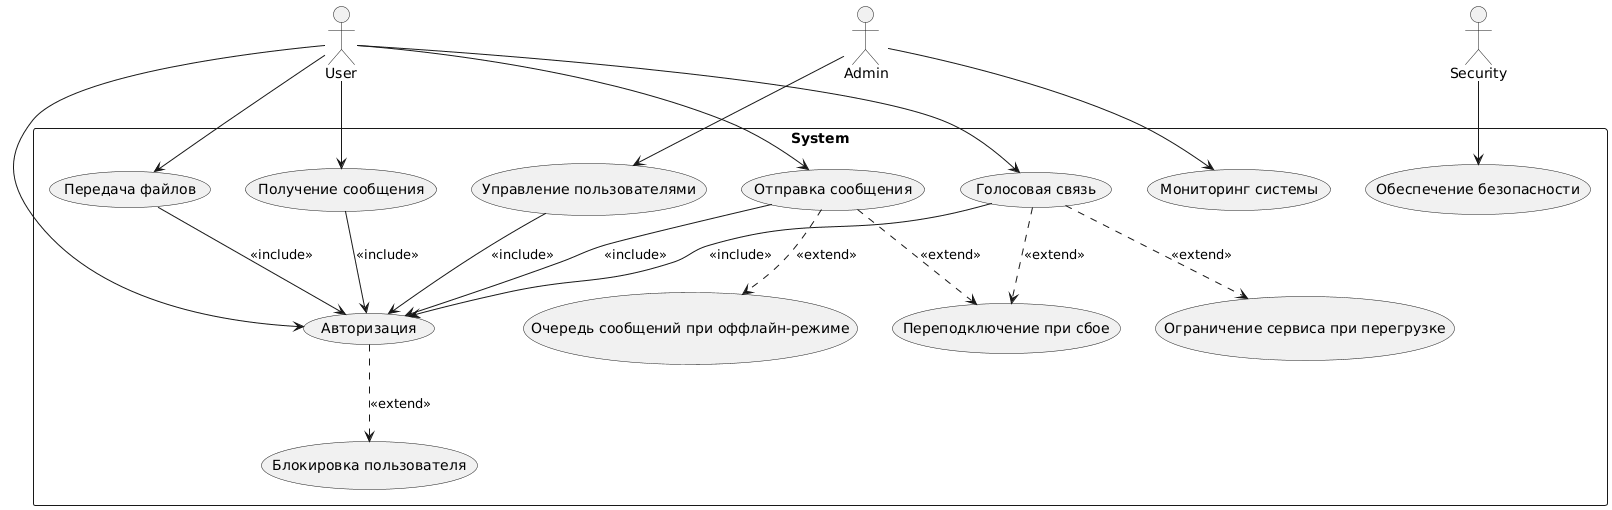
\includegraphics[width=0.78\textwidth]{usecase.png}
    \refstepcounter{figure}
    \caption*{Рисунок \thefigure\ — Диаграмма вариантов использования}
\end{figure}


\section{Описание основных вариантов использования}

\subsection{UC1: Авторизация пользователя}
Данный вариант использования описывает процесс входа пользователя в систему. Пользователь вводит учетные данные (логин и пароль), после чего система выполняет их проверку через сервер аутентификации. При успешной проверке создаётся активная сессия пользователя, и ему предоставляется доступ к функционалу системы.

Альтернативный сценарий возникает при ошибке ввода учетных данных. В этом случае система отклоняет попытку входа и запрашивает повторный ввод. Исключительный сценарий связан с блокировкой пользователя системой безопасности, при которой доступ полностью запрещается.

\subsection{UC2: Отправка текстового сообщения}
В рамках данного сценария пользователь формирует текстовое сообщение и отправляет его другому пользователю или в канал. Сообщение передаётся через сервер, который выполняет маршрутизацию и доставку получателю в режиме реального времени.

Альтернативным сценарием является ситуация, при которой получатель находится офлайн. В этом случае сообщение сохраняется в очереди доставки и передаётся при восстановлении соединения. Исключительный сценарий связан с потерей сетевого соединения, при котором отправка отклоняется или повторяется после восстановления связи.

\subsection{UC3: Голосовая связь}
Пользователь подключается к голосовому каналу, после чего система устанавливает потоковое соединение между участниками. Передача аудиоданных осуществляется в реальном времени с минимальной задержкой, оптимизированной для локальной сети.

Альтернативный сценарий включает автоматическое переподключение при кратковременном разрыве соединения. Исключительный сценарий возникает при перегрузке сети, что приводит к снижению качества связи или её разрыву.

\subsection{UC4: Передача файлов}
Пользователь инициирует передачу файла другому участнику системы. Файл разбивается на пакеты и передаётся через сервер с контролем целостности данных. Получатель принимает файл и подтверждает успешную доставку.

Альтернативным сценарием является повторная отправка пакетов при ошибках передачи. Исключительный сценарий связан с превышением допустимого размера файла или ограничениями политики безопасности, при которых передача отклоняется.

\section{Функциональные требования системы}

На основе диаграмм требований и вариантов использования сформированы следующие функциональные требования:

\begin{itemize}
    \item Система должна обеспечивать аутентификацию пользователей по логину и паролю.
    \item Система должна поддерживать отправку и получение текстовых сообщений в реальном времени.
    \item Система должна обеспечивать передачу голосовых данных между пользователями.
    \item Система должна поддерживать передачу файлов между участниками коммуникации.
    \item Система должна обеспечивать создание и управление чатами и каналами.
    \item Система должна реализовывать очереди доставки сообщений для оффлайн-пользователей.
    \item Система должна поддерживать автоматическое переподключение при потере соединения.
    \item Система должна обеспечивать администрирование пользователей и прав доступа.
    \item Система должна обеспечивать контроль и мониторинг состояния узлов системы.
    \item Система должна поддерживать механизмы блокировки пользователей при нарушениях безопасности.
\end{itemize}

\section{Нефункциональные требования системы}

Нефункциональные требования определяют качественные характеристики системы:

\begin{itemize}
    \item Время задержки при передаче сообщений не должно превышать допустимых значений в условиях локальной сети.
    \item Задержка голосовой связи должна быть минимальной (ориентировочно до 100 мс в LAN).
    \item Система должна обеспечивать шифрование всех передаваемых данных.
    \item Система должна функционировать внутри корпоративной сети без зависимости от внешних сервисов.
    \item Система должна обеспечивать масштабируемость за счёт добавления новых узлов без изменения архитектуры клиента.
    \item Система должна обеспечивать отказоустойчивость при выходе из строя отдельных серверных компонентов.
    \item Система должна поддерживать одновременную работу большого количества пользователей без деградации критичных функций.
    \item Система должна обеспечивать журналирование действий пользователей и событий системы для последующего анализа.
    \item Интерфейс системы должен обеспечивать минимальное время выполнения базовых операций (отправка сообщений, подключение к каналам).
\end{itemize}

\section{Вывод}
В ходе выполненного домашнего задания изучил методы обслуживания систем программного обеспечения.

\end{document}
